\documentclass[11pt]{article}
\usepackage{graphicx}
\usepackage{authblk}
\usepackage[utf8]{inputenc}
\graphicspath{/Users/georgeadams/Dropbox/005_ITP_projects/003 TPO/GIT_repo_TPOPROJECT/}


\title{Bayesian Analysis of TPO levels in Immune Thrombocytopenia}
\author[1,2]{\small George Adams}
\author[1,2]{\small Nichola Cooper}
\affil[1]{\footnotesize Imperial College London, Kensington, London SW7 2AZ}
\affil[2]{\footnotesize Hammersmith Hospital, Imperial College NHS Trust, London W12 0HS}



\date{July 2018}

\begin{document}

\maketitle

\paragraph{Introduction:} Thrombopoietin (TPO) is a haematopoietic growth factor, prodominately produced by the liver and kidneys, whose major function is in the regulation of platelet production. The exact mechanisms that regulate TPO levels are highly debated. The preeminent hypothesis is that TPO is synthesised in a constitutive manner and its concentration in the blood is determined by the total volume of platelets. The theory is that platelets bind TPO via high-affinity receptors and remove it from the circulation (the `sponge theory'). As platelet counts fall TPO levels rise, and vice-versa \cite{EtoLinkagemechanismsthrombocytopenia2016}. In patients with active ITP, however, TPO levels have been shown to have inappropriately low. This has been thought to be because the higher rate of platelet turnover in active ITP causes additional amounts of TPO to be consumed. To better understand the relationship between TPO and platelets in ITP we measured TPO levels in a 67 patients with ITP and 6 patients with aplastic anaemia, which acted as non-immune thrombocytopenic controls. We used a bayesian regresssion approach to analyse the association between TPO and platelet counts. This approach allows us to infer TPO concentration over a range of different platelet counts and has been shown to be more accurate with smaller sample sizes than classical gaussian regression models \cite{GoldsteinBayesiananalysisregression1976}.


\paragraph{Methods:} Blood samples were collected in an outpatient setting with most patients having duplicate samples. Samples were collected in sodium citrate, double spun to remove platelet fractions and then stored at -80°C within four hours of collection. Each patient had an additional full blood count at the time of collection. TPO levels were measured using quantitive sandwich enzyme immunoassay technique according to the manufacturers instructions. Optical density values were measured by microplate reader. We used log-normalised tpo and platelet counts in a bayesian regression model; $log(TPO) = alpha + beta*log(platelet)$. We used uninformative gaussian (mean 0, standard deviation 10) as our priors. We calculated posteriors distributions for a range of different platelet counts (1 to 200) and from these calculated \textit{maximium a posteriori} (MAP) estimates and 90\% Bayesian Confidence intervals (BCI).


\paragraph{Results:} Of the 130 samples collected, we excluded 30 samples which failed to detect any TPO. All but 1 patient had a second positive repeat sample available. In the ITP patients TPO levels ranged between 14-829.3pg/ml with platelet counts ranging from 4 to 452 x$10^9/L$. In our aplastic comparison group, platelet counts were equally spread over a range 4 to 132$x10^9/L$ (mean 47$x10^9/L$) with TPO levels ranging from 17 to 4572.5pg/ml. We found a non-linear relationship between platelet counts and TPO levels in both ITP and aplastic patients (FIGURE 1). In our ITP patients, for a given platelet count of 1 the MAP estimate was 410pg/ml (BCI; 200-804pg/ml). This declined sharply to 100pg/ml as the platelet count increased to 10$x10^9/L$. At platelet counts of 50$x10^9/L$ the TPO levels stabilised with a MAP estimate of 37.5pg.ml (BCI 31 to 46pg/ml) after which decline in TPO with platelet count was much more shallow. At a platelet count of 200$x10^9/L$ our MAP estimate was 16pg/ml (BCI 11-21 pg/ml) for this ITP group. TPO levels in our comparison aplastic group consistently higher than our ITP patients, irrespective of platelet count. The peak TPO MAP estimate for this aplastic group was >10000pg/ml but fell rapidly to 572pg/ml at a platelet count of 50$x10^9/L$. At a platelet count of 100$x10^9/L$ the MAP estimate was 221pg/ml (BIC 112 to 828pg/ml). This is approaching the normal range for a healthy individual (mean 120pg/ml, range 80 - 230pg/ml) \cite{SinghCirculatingthrombopoietinlevels2015}.

\paragraph{Conclusions:} Our study identified that in patients with ITP there is a non-linear correlation between platelet count and TPO levels, with a flattening off of TPO levels at platelet counts between 50-100$x10^9/L$. The levels of TPO in these ITP patients were consistently lower than in our non-immune (aplastic) thrombocytopenic controls, irrespective of the platelet count or disease activity. These findings oppose the prevailing theory that TPO levels are determined directly by the total summated volume of platelets. It also revutes the idea that active ITP causes the lower-than-expected TPO levels observed, as this remains the case even in non-active ITP. These findings suggest that either an additional process keeps TPO levels lower in these patients or, alternatively, that there is some impairment of TPO synthesis in ITP.



%\begin{center}
% \begin{tabular}{||c c c c c||}
% \hline\hline
%  ITP   & platelet count & MAP & lower BCI & Upper BCI  \\
%\hline\hline
% Platelet count & 1 & 410 & 200  & 804 \\
% \hline
% Patelet count & 10 & 100 &  75 & 151 \\
% \hline
% Platelet count & 50 & 37.5 & 31 & 46 \\
% \hline
% Platelet count & 200 & 16 & 11 & 21 \\ [1ex]
% \hline
%\end{tabular}
%\end{center}

\begin{figure}
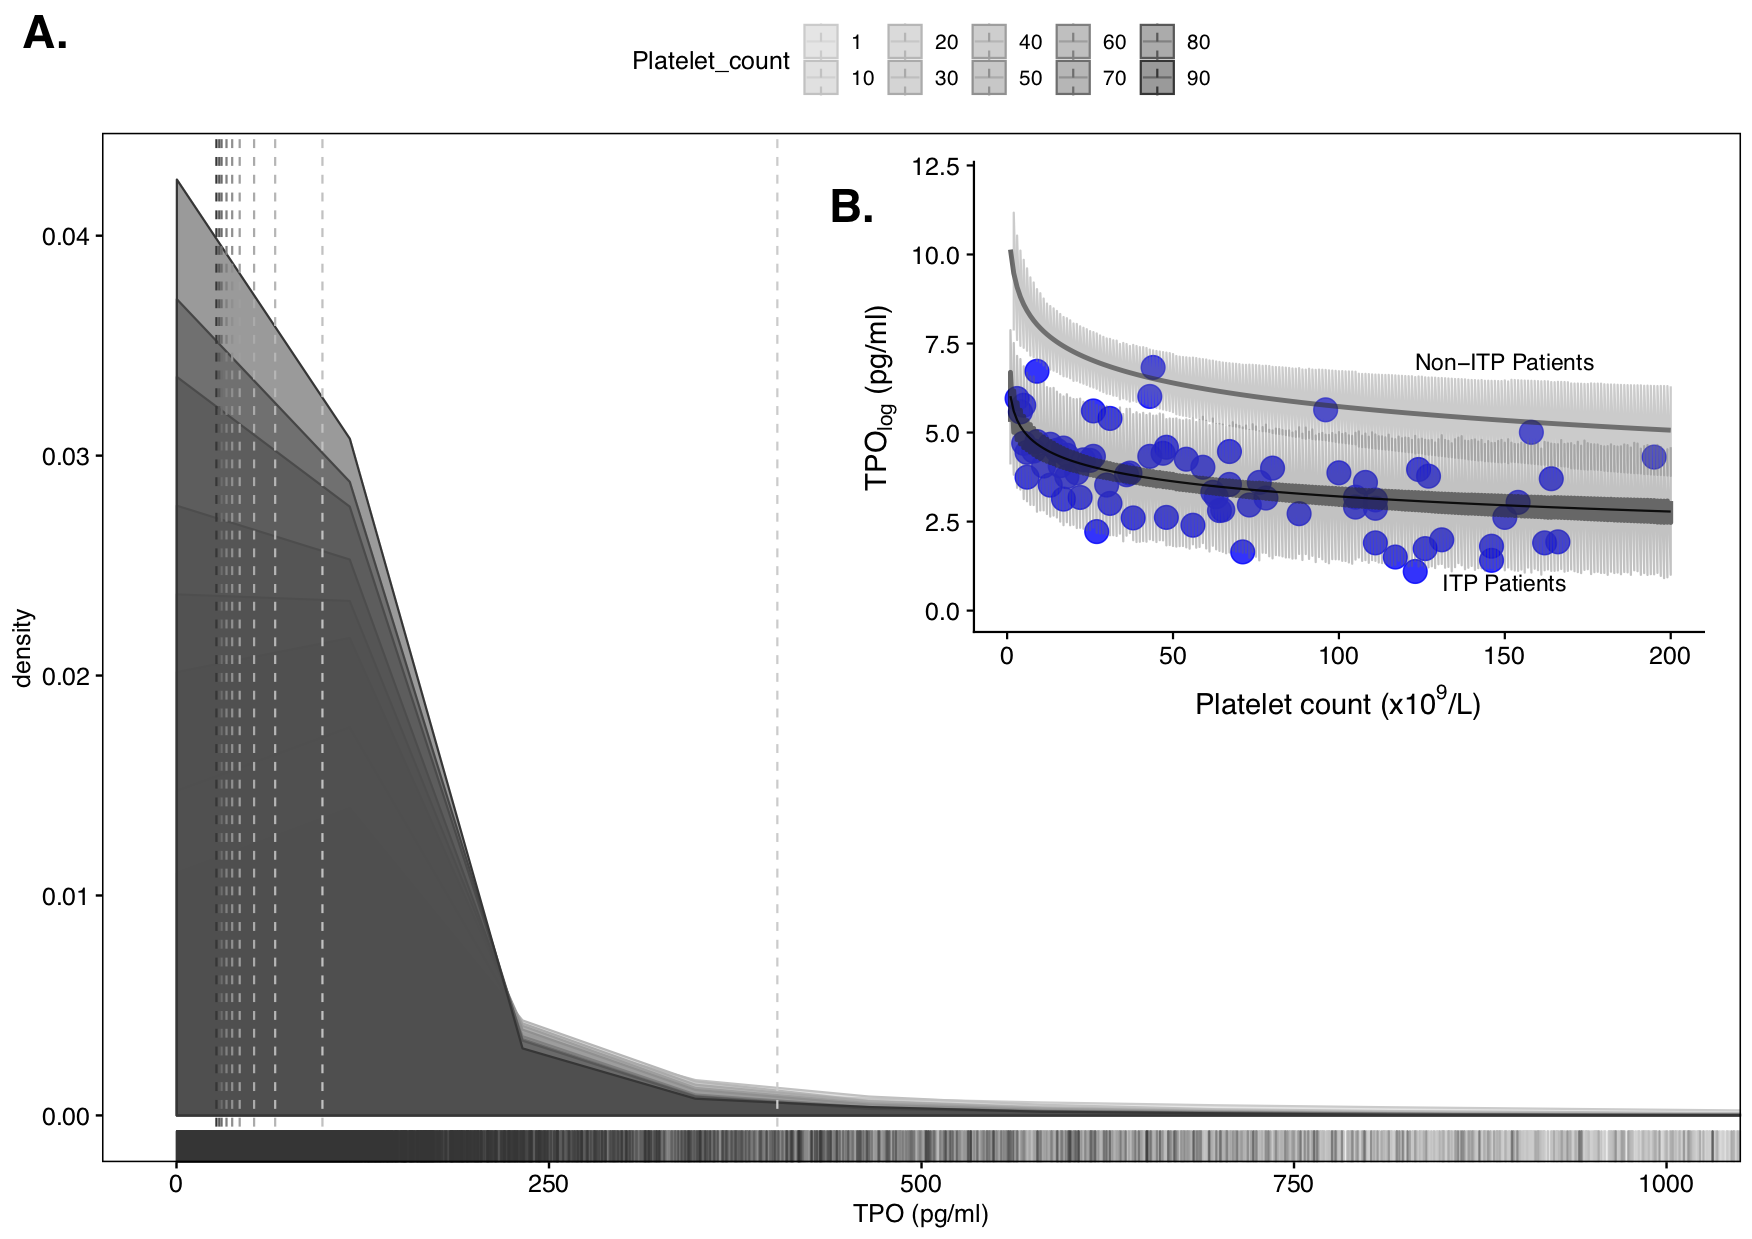
\includegraphics[]{ABSTRACT_v3_graph1.png}
\caption {FIGURE 1: A.) Shows posterior probabiltiy distributions for different platelet counts ranging from 1 to 90 in our ITP patient group. Dashed vertical lines represent \textit{maximium a posteriori} (MAP) estimates for each distribution, moving from right to left as platelet counts increase and TPO levels falls. B.) Curved lines with shading shows model predictions for logTPO levels versus platelet counts in both ITP patients (lower line) and Aplastic controls (upper line). Points represent the individual results for the ITP group. Darker shaded area represent the 90\% bayesian credible interval and the lighter shading represents the simulated observational interval. Points are the results our ITP patients only.}
\end{figure}

\bibliographystyle{plain}
\bibliography{tpobib.bib}


\paragraph{}
\textbf{Currently 4504 characters - needs to be characters: 3800}


\end{document}
